% Documentación de la Etapa 5
% Compilar con:  pdflatex Informe_etapa5.tex
\documentclass[11pt,a4paper]{article}

\usepackage[utf8]{inputenc}
\usepackage[margin=2.5cm]{geometry}
\usepackage{url}
\usepackage{graphicx}
\usepackage{tikz}
\usepackage{float}

\title{Etapa 5 - Generación de Código CeIVM de MiniJava}
\author{Compiladores e Intérpretes --- UNS, 2026}
\date{}

% Esta instalacion TeX puede no tener las fuentes TS1 (text companion): se evitan
% los simbolos que las requieren (vinetas de itemize, llaves via \{ en \texttt).
\renewcommand{\labelitemi}{$\bullet$}

\begin{document}

\sloppy

\maketitle

\noindent
Implementación del Generador de Código de MiniJava. Se extiende el trabajo de la
Etapa 4 (ASTs y chequeo de sentencias) para que, una vez verificadas las
declaraciones y las sentencias, el compilador calcule los desplazamientos en los
registros de activación, en los CIR y en las tablas virtuales, recorra la Tabla de
Símbolos y los AST y emita el programa en código intermedio CeIASM que ejecuta la
máquina virtual CeIVM. El módulo principal escribe ese código en un archivo de
salida cuyo nombre indica el usuario. La generación cubre, además, los controles
y representaciones que el apunte de la CeIVM exige para la semántica base
(punto de entrada, arreglos y Strings). No se implementan logros de la etapa.

\section{Objetivo y logros}

\begin{itemize}
  \item Extender la Tabla de Símbolos y los nodos del AST con métodos que generen
        el código CeIASM correspondiente a su significado.
  \item Calcular, como parte del análisis semántico, los offsets de atributos (en
        el CIR), de métodos de instancia (en la VT) y de parámetros y variables
        locales (en el RA), teniendo en cuenta la herencia.
  \item Agregar al módulo principal la generación del archivo de salida con el
        código intermedio, cuyo nombre recibe por parámetro, y mantener el
        reporte de errores y el mensaje \texttt{[SinErrores]}.
  \item Controlar el punto de entrada cuando se genera código: exactamente un
        método \texttt{static void main()} sin parámetros.
  \item Emitir los controles en tiempo de ejecución que el apunte exige para los
        arreglos (índice fuera de rango y tamaño negativo) y representar los
        Strings como objetos del \texttt{.heap}.
\end{itemize}

Se mantienen los logros de etapas anteriores que siguen vigentes (atributos
inicializados, operadores posfijos, visibilidad mejorada, manejo de archivos
eficiente y genericidad avanzada de las Etapas 2 y 3). \textbf{No se intentan
logros de la Etapa 5}: no se implementan floats ni coerción, \texttt{for},
ternario, \texttt{super}, herencia múltiple de interfaces, \texttt{toString} real
ni minilambdas. La sintaxis de escapes \texttt{\textbackslash uXXXX} tampoco se
resuelve (logro de la Etapa 1).

\section{Esquema general}

El módulo principal recibe el archivo fuente y el nombre del archivo de salida.
Como en la Etapa 4, asocia el fuente al manejador de archivos y este al léxico,
crea la \texttt{TablaDeSimbolos} y el \texttt{AnalizadorSintactico}, y dispara el
análisis. Al finalizar el parseo ejecuta el chequeo de declaraciones
(\texttt{estaBienDeclarada}), la consolidación (\texttt{consolidar}) y el chequeo
de cuerpos (\texttt{chequearCuerpos}). Si se pidió un archivo de salida, controla
el punto de entrada (\texttt{chequearPuntoDeEntrada}) y luego solicita a la tabla
el código generado (\texttt{generarCodigo}), lo escribe en el archivo de salida y
reporta el éxito. Ante un error léxico, sintáctico o semántico reporta el mensaje
y el código de error y finaliza.

\begin{figure}[H]
\centering
\resizebox{\textwidth}{!}{%
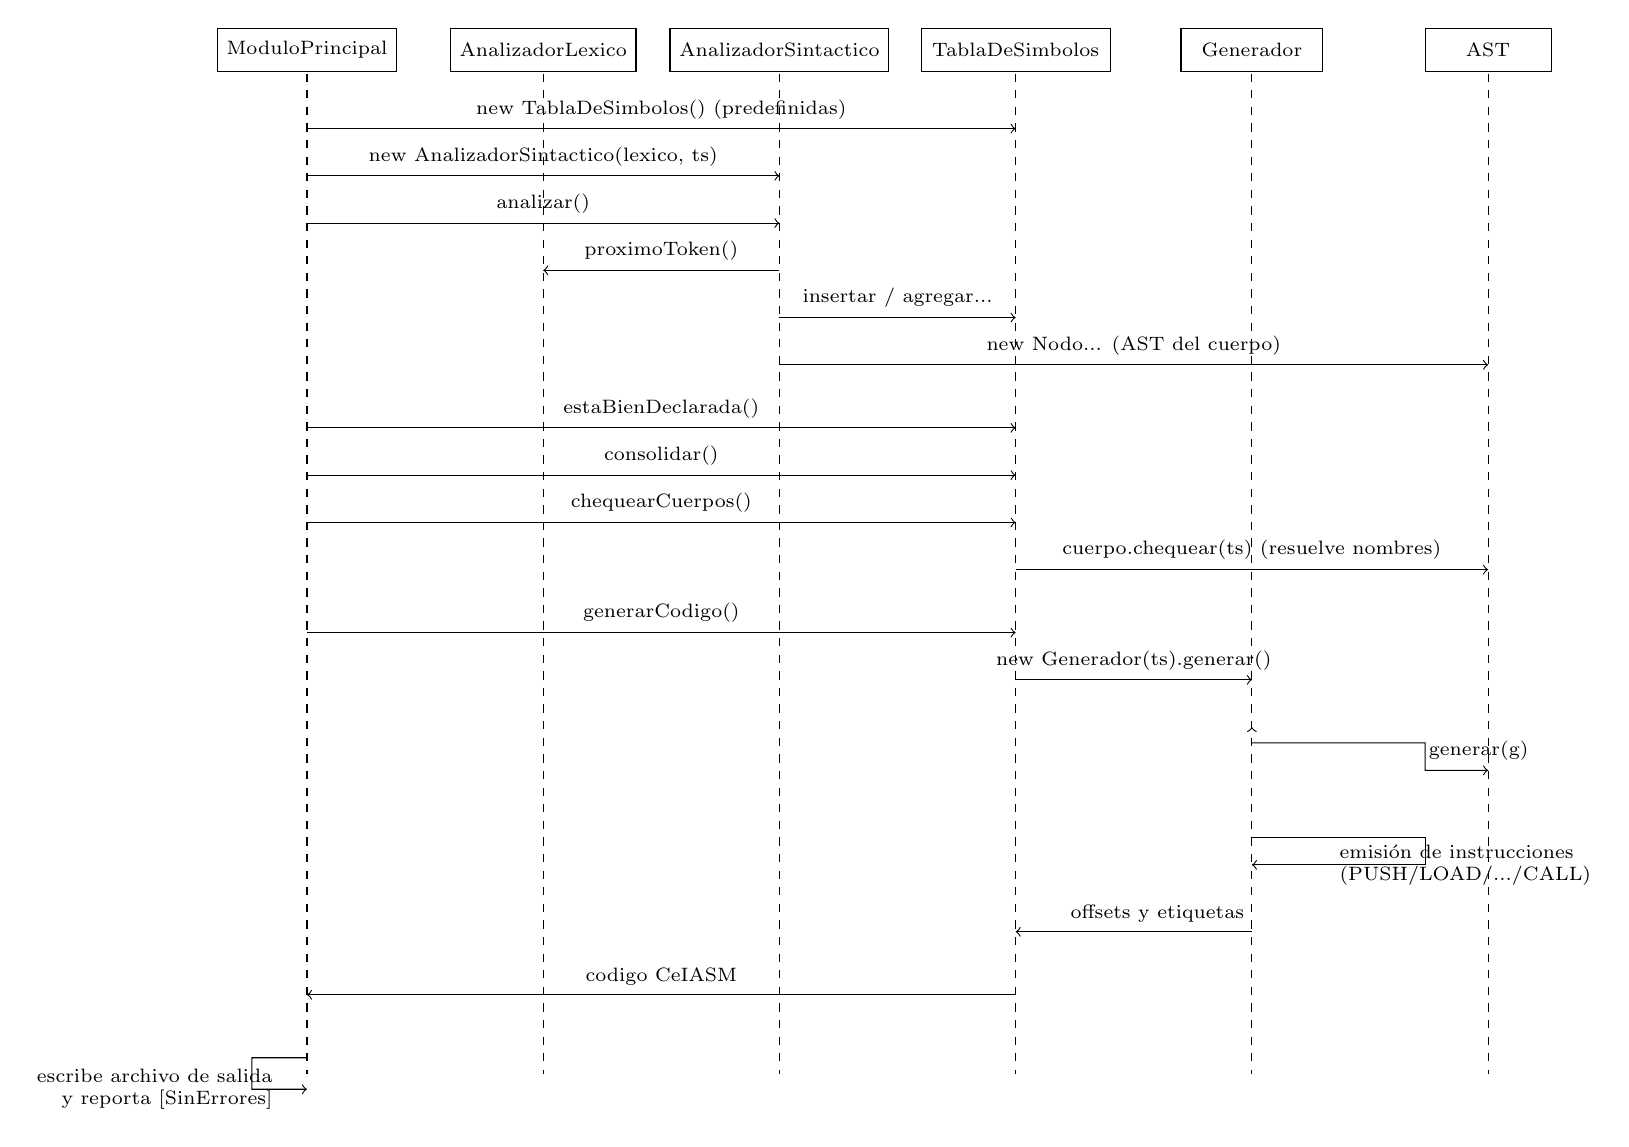
\begin{tikzpicture}[font=\scriptsize]
\def\MP{0}\def\AL{3.0}\def\AS{6.0}\def\TS{9.0}\def\GEN{12.0}\def\AST{15.0}
% participantes
\node[draw,minimum width=2.0cm,minimum height=0.55cm] (mp) at (\MP,0) {ModuloPrincipal};
\node[draw,minimum width=2.0cm,minimum height=0.55cm] (al) at (\AL,0) {AnalizadorLexico};
\node[draw,minimum width=2.4cm,minimum height=0.55cm] (as) at (\AS,0) {AnalizadorSintactico};
\node[draw,minimum width=2.4cm,minimum height=0.55cm] (ts) at (\TS,0) {TablaDeSimbolos};
\node[draw,minimum width=1.8cm,minimum height=0.55cm] (gen) at (\GEN,0) {Generador};
\node[draw,minimum width=1.6cm,minimum height=0.55cm] (ast) at (\AST,0) {AST};
% lineas de vida
\foreach \x in {\MP,\AL,\AS,\TS,\GEN,\AST} { \draw[dashed] (\x,-0.3) -- (\x,-13.0); }
% mensajes
\draw[->] (\MP,-1.0) -- (\TS,-1.0) node[midway,above,align=center]{new TablaDeSimbolos() (predefinidas)};
\draw[->] (\MP,-1.6) -- (\AS,-1.6) node[midway,above,align=center]{new AnalizadorSintactico(lexico, ts)};
\draw[->] (\MP,-2.2) -- (\AS,-2.2) node[midway,above,align=center]{analizar()};
\draw[->] (\AS,-2.8) -- (\AL,-2.8) node[midway,above,align=center]{proximoToken()};
\draw[->] (\AS,-3.4) -- (\TS,-3.4) node[midway,above,align=center]{insertar / agregar...};
\draw[->] (\AS,-4.0) -- (\AST,-4.0) node[midway,above,align=center]{new Nodo... (AST del cuerpo)};
\draw[->] (\MP,-4.8) -- (\TS,-4.8) node[midway,above,align=center]{estaBienDeclarada()};
\draw[->] (\MP,-5.4) -- (\TS,-5.4) node[midway,above,align=center]{consolidar()};
\draw[->] (\MP,-6.0) -- (\TS,-6.0) node[midway,above,align=center]{chequearCuerpos()};
\draw[->] (\TS,-6.6) -- (\AST,-6.6) node[midway,above,align=center]{cuerpo.chequear(ts) (resuelve nombres)};
\draw[->] (\MP,-7.4) -- (\TS,-7.4) node[midway,above,align=center]{generarCodigo()};
\draw[->] (\TS,-8.0) -- (\GEN,-8.0) node[midway,above,align=center]{new Generador(ts).generar()};
\draw[->] (\GEN,-8.6) -- (\GEN,-8.6);
\draw[->] (\GEN,-8.8) -- ++(2.2,0) -- ++(0,-0.35) -- (\AST,-9.15)
    node[midway,above,align=center,pos=0.85]{generar(g)};
\draw[->] (\GEN,-10.0) -- ++(2.2,0) -- ++(0,-0.35) -- (\GEN,-10.35)
    node[right,align=left,pos=0.55]{emisión de instrucciones\\(PUSH/LOAD/.../CALL)};
\draw[->] (\GEN,-11.2) -- (\TS,-11.2) node[midway,above,align=center,pos=0.4]{offsets y etiquetas};
\draw[->] (\TS,-12.0) -- (\MP,-12.0) node[midway,above,align=center]{codigo CeIASM};
\draw[->] (\MP,-12.8) -- ++(-0.7,0) -- ++(0,-0.4) -- (\MP,-13.2)
    node[left,align=right,pos=0.55]{escribe archivo de salida\\y reporta [SinErrores]};
\end{tikzpicture}%
}
\caption{Diagrama de secuencia de la Etapa 5.}
\end{figure}

\section{Cálculo de offsets y etiquetas}

El cálculo se realiza en una pasada posterior a la consolidación (por lo tanto,
con los miembros heredados ya incorporados) y previa a la generación. Como los
offsets de un miembro dependen de los de sus ancestros, las clases y las
interfaces se procesan recursivamente desde \texttt{Object}.

\begin{itemize}
  \item \textbf{CIR (atributos).} El desplazamiento 0 es la referencia a la VT y
        los atributos ocupan desde el 1. Los atributos heredados conservan el
        desplazamiento que tenían en el ancestro; los propios se numeran a
        continuación en orden de declaración.
  \item \textbf{VT (métodos de instancia).} El desplazamiento 0 es
        \texttt{Object.toString} y los métodos de instancia ocupan desde el 1. Los
        métodos estáticos no ocupan entradas. Una clase que extiende a otra copia
        la VT del ancestro: las redefiniciones reutilizan la entrada heredada y
        los métodos nuevos se agregan al final. Una clase que implementa una
        interfaz (o una interfaz que extiende a otra) comienza con
        \texttt{[toString]} seguida por los métodos de la interfaz en su orden de
        declaración, de modo que el desplazamiento coincide en la interfaz y en
        todas las clases que la implementan.
  \item \textbf{RA (parámetros y variables locales).} Para una unidad con $n$
        parámetros: en una unidad estática el parámetro $i$ está en $n+3-i$ y la
        celda de resultado en $n+3$; en una unidad de instancia (y en los
        constructores) \texttt{this} está en 3, el parámetro $i$ en $n+4-i$ y la
        celda de resultado en $n+4$. Las variables locales reciben, durante la
        generación, los desplazamientos $0,-1,-2,\dots$ según quedan vivas.
\end{itemize}

Las etiquetas del código se construyen a partir del nombre de la unidad, su
aridad y la clase que la declara: \texttt{lblMet<nombre>\_<aridad>@<Clase>} para
los métodos y \texttt{lblConstructor\_<aridad>@<Clase>} para los constructores,
de modo que una redefinición conserva la etiqueta de la versión declarada en cada
clase.

El lenguaje CeIASM no distingue mayúsculas de minúsculas, por lo que dos nombres
que sólo difieren en el \emph{casing} (por ejemplo \texttt{getX} y \texttt{getx}
en una misma clase, o las clases \texttt{Foo} y \texttt{FOO}) producirían
etiquetas colisionantes. Para evitarlo, todo nombre se codifica anteponiendo un
\texttt{\$} a cada letra mayúscula antes de formar la etiqueta (también la de la
VT, \texttt{lblVT<Clase>}). El \texttt{\$} no puede aparecer en un identificador
MiniJava y sí es válido en una etiqueta CeIASM, de modo que la codificación es
inyectiva aun ignorando el casing.

\section{Estructura del código generado}

El programa CeIASM generado tiene la siguiente estructura:

\begin{enumerate}
  \item \textbf{Entry point.} Bajo \texttt{.CODE}: la llamada a
        \texttt{simple\_heap\_init}, la llamada al método \texttt{main} y la
        instrucción \texttt{HALT}.
  \item \textbf{Rutinas de gestión del heap.} \texttt{simple\_heap\_init} y
        \texttt{simple\_malloc}, tomadas del esquema simplificado del apunte.
  \item \textbf{Rutinas de error.} \texttt{lErrorIndice} y
        \texttt{lErrorTamanio} imprimen con \texttt{SPRINT} el mensaje
        correspondiente y ejecutan \texttt{HALT}; los mensajes se reservan en
        \texttt{.DATA}.
  \item \textbf{Por cada clase}: en \texttt{.DATA} su tabla virtual
        (\texttt{lblVT<Clase>: DW ...}), que contiene las etiquetas de los métodos
        de instancia en el orden de la VT; y bajo \texttt{.CODE} el código de su
        constructor y de sus métodos.
  \item \textbf{Entidades predefinidas.} Se generan \texttt{Object},
        \texttt{String} y \texttt{System} con sus VT, constructores vacíos y
        métodos (\texttt{debugPrint} con \texttt{IPRINT}, \texttt{toString},
        \texttt{read} con \texttt{READ}, \texttt{printB/C/I/S},
        \texttt{println} y sus variantes con salto de línea).
  \item \textbf{Strings literales.} No se guardan en \texttt{.DATA}: cada
        evaluación construye en el \texttt{.heap} un bloque
        \texttt{[VT, longitud, caracteres..., 0]} y deja su referencia en la pila.
\end{enumerate}

\section{Traducciones}

Por cada unidad se genera un prólogo (\texttt{LOADFP; LOADSP; STOREFP}), el
cuerpo del AST y un epílogo (\texttt{FMEM} de las locales vivas,
\texttt{STOREFP} y \texttt{RET} con el número de celdas a liberar: $n$ en
unidades estáticas y $n+1$ en unidades de instancia y constructores).

\begin{center}
\footnotesize
\begin{tabular}{ll}
\hline
Construcción & Código \\
\hline
literal int/char/bool/null & \texttt{PUSH k} (char a ASCII, bool a 1/0, null a 0) \\
literal string & construcción del String en el \texttt{.heap} \\
variable local / parámetro & \texttt{LOAD off} \\
atributo & \texttt{LOAD 3; LOADREF off} \\
\texttt{this} & \texttt{LOAD 3} \\
binaria & código de los hijos + ADD/SUB/MUL/DIV/MOD/LT/GT/LE/GE/EQ/NE \\
\texttt{\&\&} y \texttt{||} & cortocircuito con BF/BT y normalización a 1/0 \\
unaria & \texttt{NEG} / \texttt{NOT} (el + no genera instrucción) \\
\texttt{a.length} & código de \texttt{a} + \texttt{LOADREF 1} \\
\texttt{a[i]} & código de \texttt{a} y de \texttt{i}, control de rango, \texttt{ADD}, \texttt{LOADREF 2} \\
asignación & código del lado derecho, \texttt{DUP}, destino \\
\texttt{new C(args)} & \texttt{RMEM 1; PUSH k; PUSH simple\_malloc; CALL; DUP;} \\
 & \texttt{PUSH lblVT<C>; STOREREF 0; DUP;} args con \texttt{SWAP}; \\
 & \texttt{PUSH lblConstructor@<C>; CALL} \\
llamada estática & \texttt{RMEM 1} (si retorna), args, \texttt{PUSH etiq; CALL} \\
llamada de instancia & receptor, \texttt{RMEM 1}, \texttt{SWAP}, args con \texttt{SWAP}, \\
 & \texttt{DUP; LOADREF 0; LOADREF offVT; CALL} \\
\texttt{if} & condición, \texttt{BF else}, rama, \texttt{JUMP fin}, \texttt{else:}, \texttt{fin:} \\
\texttt{while} & \texttt{ini:}, condición, \texttt{BF fin}, cuerpo, \texttt{JUMP ini}, \texttt{fin:} \\
\texttt{return E} & \texttt{E}, \texttt{STORE retval}, epílogo \\
sentencia expresión & expresión; \texttt{POP} si deja valor \\
\texttt{var x = E} & código de \texttt{E} (cae en la celda de \texttt{x}) \\
\hline
\end{tabular}
\end{center}

La referencia al objeto actual se apila con \texttt{LOAD 3} (o se recibe como
receptor), y el acceso a un atributo usa \texttt{LOADREF} con su offset en el
CIR; la asignación a un atributo reevalúa el receptor, \texttt{SWAP} y
\texttt{STOREREF}. En los métodos de instancia la referencia al receptor forma
parte del RA (desplazamiento 3). Los arreglos se representan como objetos del
heap con la VT de \texttt{Object} en el desplazamiento 0 y la longitud en el 1.

Cada unidad reserva al entrar un conjunto fijo de celdas temporales
(\texttt{RMEM TAM\_POOL}) que el generador entrega con
\texttt{reservarTemporal}/\texttt{liberarTemporal}. Al tener un desplazamiento
fijo en el RA, estas celdas sirven aunque la pila de expresiones no esté vacía
(por ejemplo, al crear un arreglo como argumento). Los arreglos de cualquier
cantidad de dimensiones se construyen evaluando y controlando primero todos los
tamaños y recorriendo luego, con un ciclo anidado por dimensión, las componentes
de cada nivel para alojar los subarreglos.

El acceso a una componente controla el índice negativo y el índice mayor o igual
que la longitud (y la referencia nula, al leer la longitud con \texttt{LOADREF
1}); si falla, salta a \texttt{lErrorIndice}. La creación controla cada dimensión
negativa y salta a \texttt{lErrorTamanio}. Los literales String se construyen en
el \texttt{.heap} en cada evaluación, de modo que dos literales iguales son
objetos distintos; \texttt{System.printS*} suma el desplazamiento 2 antes de
\texttt{SPRINT}.

\section{Formato de salida}

\subsection{Análisis exitoso}

{\footnotesize
\begin{verbatim}
Compilacion Exitosa
[SinErrores]
\end{verbatim}
}

y se escribe en el archivo de salida el programa CeIASM. El archivo puede
ejecutarse con \texttt{java -jar CeIVM-cei2011.jar <archivo>}.

\subsection{Análisis con errores}

El comportamiento no cambia respecto de las etapas anteriores: se muestra un
mensaje descriptivo y el código \texttt{[Error:lexema|nroLinea]}.

\section{Compilación y ejecución}

No se usa ninguna herramienta de build: solo se necesitan \texttt{javac},
\texttt{jar} y \texttt{java} de cualquier JDK 21 o superior (probado con JDK 25).

{\footnotesize
\begin{verbatim}
./Compilar.sh             # compila y genera Compilador.jar  (Windows: Compilar.bat)
java -jar Compilador.jar recursos/sinErrores/gen-01.java salida.txt
java -jar CeIVM-cei2011.jar salida.txt
./CorrerTests.sh          # compila y ejecuta los testers JUnit  (Windows: CorrerTests.bat)
\end{verbatim}
}

El primer parámetro del compilador es el archivo fuente (con cualquier extensión)
y el segundo es el archivo de salida (también con cualquier extensión; si se
omite, el compilador solo analiza, sin generar código).

\section{Tests}

Se incluyen:
\begin{itemize}
  \item los cuatro casos provistos por la cátedra (\texttt{gen-01} a
        \texttt{gen-04}), que se ejecutan con la CeIVM y comparan su salida;
  \item una batería propia de casos de generación (\texttt{gen-05} a
        \texttt{gen-110}) que cubren expresiones, variables locales,
        parámetros, aritmética, lógica, atributos, herencia, interfaces
        (simples y extendidas), constructores, \texttt{new}, arreglos
        unidimensionales y multidimensionales, encadenados, strings, caracteres,
        \texttt{if}, \texttt{while}, \texttt{return}, recursividad, llamadas
        estáticas, de instancia e implícitas, \texttt{this}, genéricos y
        despacho dinámico, además de los errores de ejecución (índice fuera de
        rango, tamaño negativo, referencia nula y división por cero);
  \item los casos del punto de entrada de la etapa y los errores semánticos de
        las etapas anteriores (\texttt{resources/conErrores/}), que deben
        rechazarse.
\end{itemize}

El resultado de la ejecución de \texttt{./CorrerTests.sh} es \textbf{OK (191
tests)}. Los casos de generación se ejecutan con la CeIVM desde el tester: por
cada caso se genera \texttt{[caso].out} y se compara la salida de la máquina
virtual con la indicada en la primera línea del archivo fuente (formato
\texttt{///valor1\&valor2\&...\&exitosamente}).

\section{Fuera de alcance (logros)}

No se implementaron los logros de la etapa: floats y coerción (concatenación de
strings incluida), \texttt{for} clásico y de iteradores, ternario, \texttt{super},
herencia múltiple de interfaces, \texttt{toString} real ni minilambdas. La
sintaxis aceptada sigue siendo la de las etapas anteriores (tampoco se resuelven
los escapes \texttt{\textbackslash uXXXX}); la generación cubre la semántica base
de MiniJava, incluidos el punto de entrada, los controles de arreglos y la
representación de Strings del apunte.

\end{document}
